
% Last updated: ~ August 2020 (Khan Academy)
% I probably typeset this for no reason or made a minor change on December 13, 2020.
\documentclass[11pt]{article}   


\usepackage{amsfonts}
\usepackage{amsmath} 
\usepackage{amssymb}
\usepackage{amsthm}
\usepackage{enumitem}
\usepackage{geometry}    
\usepackage{graphicx}	
\usepackage{indentfirst}
\usepackage[utf8]{inputenc}
\usepackage{parcolumns}
\usepackage{polynom}
\usepackage{tikz}
\usepackage[T1]{fontenc}
\usepackage{tikz-cd}

\usepackage{esint}
 \usepackage{pgfplots}
 
 
 \setlength{\textwidth}{6.5in}
\setlength{\oddsidemargin}{-0.1in}
\setlength{\evensidemargin}{-0.1in}

 

 \theoremstyle{definition}
\newtheorem{ex}{Example}[section]



\newcommand{\nc}{\newcommand} % makes for easier new commands
\nc{\ba}{\begin{align*}} % beginning aligned 
\nc{\bb}{\mathbb} % blackboard bold (fields)
\nc{\be}{\begin{equation}} % beginning equation
\nc{\ben}[1]{\begin{enumerate}[label=({#1})]} % beginning enumeration (arg: type)
\nc{\bmx}[4]{\begin{bmatrix} {#1} & {#2} \\ {#3} & {#4} \\ \end{bmatrix}} % bracketed matrix
\nc{\Bmx}[4]{\begin{Bmatrix} {#1} & {#2} \\ {#3} & {#4} \\ \end{Bmatrix}} % braced matrix
\nc{\bp}{\begin{proof}} % beginning proof
\nc{\ea}{\end{align*}} % ending aligned
\nc{\ee}{\end{equation}} % ending equation
\nc{\een}{\end{enumerate}} % ending enumeration
\nc{\ep}{\end{proof}} % ending proof
\nc{\f}{\displaystyle\frac} % fractions
\nc{\hka}{\hookrightarrow}
\nc{\ift}{\infty} % infinity
\nc{\lf}{\left} % adjusting sizes
\nc{\lm}[2]{\displaystyle\lim_{{#1}\rightarrow{#2}}} % limit (args: variable, approaching value)
\nc{\mb}{\mathbf} % boldface
\nc{\mc}{\mathcal} % calligraphic font
\nc{\mf}{\mathfrak} % Fraktur font
\nc{\mO}{\mc{O}} % \mathcal{O}
\nc{\mx}[4]{\begin{matrix} {#1} & {#2} \\ {#3} & {#4} \\ \end{matrix}} % matrix
\nc{\pmx}[4]{\begin{pmatrix} {#1} & {#2} \\ {#3} & {#4} \\ \end{pmatrix}} % parenthetical matrix
\nc{\ra}{\rightarrow} % right arrow
\nc{\rt}{\right} % adjusting sizes		
\nc{\divg}{\nabla\cdot}
\nc{\curl}{\nabla\times}
\nc{\cross}{\times}	
\nc{\ihat}{\hat{\imath}}
\nc{\jhat}{\hat{\jmath}}
\nc{\khat}{\hat{k}}
\nc{\vect}[2]{\left[\begin{array}{c}  {#1} \\ {#2} \end{array}\right]}
\nc{\diff}[1]{\, d #1}
\nc{\fmat}[4]{\left[\begin{array}{cc}  {#1} & #2 \\ {#3}  & #4  \end{array}\right]}
\nc{\cdet}[3]{\det\left(\begin{array}{ccc} \ihat & \jhat & \khat \\ \partial_x & \partial_y & \partial_z \\ #1 & #2 & #3\end{array} \right)}
\nc{\cdets}[6]{\det\left(\begin{array}{ccc} \ihat & \jhat & \khat \\  #1 & #2 & #3\\ #4 & #5 & #6 \end{array} \right)}
\nc{\pars}[1]{\left( #1 \right)}

\title{Multivariable Calculus}
\author{Jack DeSerrano}
\begin{document}
\maketitle
\tableofcontents

\section{Derivatives of multivariable functions}


\subsection{The partial derivative}
 \textit{Partial derivatives} are derivatives for multivariable functions. Fundamentally, derivatives and partial derivatives answer the same question: how does a little nudge in one direction affect the output? Rather than using $d$ to denote the differential, we use $\partial$ to represent the partial differential. Herein, to denote the partial derivative of $f$ with respect to $x$, we will write $ \partial_x f$. 
 
 
\begin{ex}Suppose
$$
f(x,\, y) = x^2\, y + \sin y.
$$
To take the partial derivative of $f$ with respect to $y$, we treat $x$ as a constant and compute the derivative normally:
$$
 \partial_y f = x^2 +\cos y.
$$\end{ex}

The partial derivative has a formal definition. With a two-variable function $f$ evaluated at $a$ and $b$,
$$
 \partial_x f (a,\, b) \equiv \lm{h}{0}\frac{f(a+h,\, b) - f(a,\, b)}{h}.
$$
Notice the similarity between this definition and the definition of the derivative.


If we take the partial derivative of a multivariable function with respect to $x$, and then take the partial derivative of our result with respect to $y$, we will, for all intents and purposes herein, wind up with the same result as taking the partial derivative with respect to $y$ first, then $x$. Notationally, we write this as, for a function $f$,
$$
 \partial_{xy}f \equiv  \partial_{yx}f.
$$
This is known as the \textit{symmetry of second partial derivatives}.




\subsection{Gradient and the directional derivative}
\begin{ex}Suppose
$$
f(x,\, y) = x^2\, \sin y.
$$
Taking the partial derivatives of $f$ with respect to $x$ and $y$,
$$
\begin{aligned}
& \partial_x f = 2x\,\sin y,\\
& \partial_y f = x^2\,\cos y.
\end{aligned}
$$
The \textit{gradient} of $f$ outputs a vector of the partial derivatives of $f$:
$$
\nabla f = \left[\begin{array}{c}2x\,\sin y \\x^2\,\cos y\end{array}\right]
$$
where $\nabla$, pronounced \textit{nabla} or \textit{del}, is the gradient operator. \end{ex}


For any function $f$ with $n$ dimensions and $x_i$ representing the $i$th input of the function, 
$$
\nabla f \equiv \left[\begin{array}{c}f_{x_1} \\f_{x_2}\\\vdots\\f_{x_n}\end{array}\right].
$$
Therefore, think of the gradient operator as the full derivative; it captures all of the partial derivatives of a multivariable function.


The \textit{directional derivative} of a function is the rate at which the function $f$ changes at a point in the direction of a vector $\mb{v}$. This directional derivative is denoted $\nabla_\mb{v} f$. To calculate the directional derivative of a function $f$ in the direction $\mb{v}$, we take the dot product of the vector and the function's gradient:
$$
\nabla_\mb{v} f\equiv\mb{v}\cdot\nabla f.
$$
Normalize $\mb{v}$ so that its magnitude is 1 when computing slope.


The directional derivative's formal definition is as follows, where $\mb{x}$ is the input point.
$$
\nabla_\mb{v} f(\mb{x}) \equiv \lm{h}{0}\frac{f(\mb{x}+h\mb{v}) - f(\mb{x})}{h}.
$$


From a graphical perspective, the gradient points in the direction of steepest ascent from a point.
\bp
The above proposition is equivalent to asking what unit vector $\mb{v}$ maximizes
$$
\nabla f(a,\, b) \cdot \mb{v}
$$
for the gradient of a function $f$ at a point $(a,\, b)$. Consider the figure below, which illustrates the above dot product.
$$
\begin{tikzpicture}
\draw[->] (0,0)--(4,0) node[right]{$x$};
\draw[->] (0,0)--(0,4) node[above]{$y$};
\draw[-stealth](1,1)--(3,3) node[anchor=south]{$\nabla f(a,\, b) $};
\draw[-stealth, red](1,1)--(2,1) node[anchor=west]{$\mb{v} $};
\draw[dashed](2,1)--(1.5,1.5);
\draw[red](1,1)--(1.5,1.5) node[anchor=south east]{ $l $};
\end{tikzpicture}
$$
Multiplying $l$ by the magnitude of the gradient vector carries the same meaning as dotting the vector of choice with the gradient vector. If we maximize $l$, we maximize the dot product. The projected length $l$ depends on the direction of $\mb{v}$. If we change $\mb{v}$ to have the direction of the gradient, like so, 
$$
\begin{tikzpicture}
\draw[->] (0,0)--(4,0) node[right]{$x$};
\draw[->] (0,0)--(0,4) node[above]{$y$};
\draw[-stealth](1,1)--(3,3) node[anchor=south]{$\nabla f(a,\, b) $};
\draw[-stealth, red](1,1)--(1.70710678119,1.70710678119) node[anchor=north west]{$\mb{v} $};
\draw[red](1,1)--(1.70710678119,1.70710678119) node[anchor=south east]{ $l $};
\end{tikzpicture}
$$
we find that $\mb{v}$'s direction maximizes $l$ by the triangle inequality or simple observation. Therefore, this dot product will be maximized when $\mb{v}$ points in the direction of the gradient vector. Thus, the gradient always points in the direction of steepest ascent.
\ep
In general, the unit vector $\mb{u}$ maximizing $\mb{u}\cdot\mb{v}$ points in the same direction as $\mb{v}$.



\subsection{The multivariable chain rule}
Suppose we have a function $f(x,\, y)$ where $x$ and $y$ are parameterized by $t$. We find that
$$
\frac{ d }{ d t}\: f(x,\, y) \equiv \partial_x f \,  \frac{ d x}{ d t} +\partial_y f \, \frac{ d y}{ d t}.
$$
Now suppose we define a vector-valued function $\mb{v}$ to contain the components of $f$. It is clear that the equality above is a dot product of a vector of the partial derivatives of $f$ and a vector of ordinary derivatives with respect to $t$. We can, therefore, write the above equality as
$$
\frac{ d }{ d t}\: f(\mb{v}) \equiv \nabla f \cdot \frac{ d \mb{v}}{ d t}.
$$
This is known as the \textit{multivariable chain rule}. It is resemblant of the single-variable chain rule.


\begin{ex} Suppose we have a two-variable function
$$
f(x,\, y) = x^2\, y
$$
where
\begin{align*}
&x = \sin t,\\
&y = \cos t.
\end{align*}
We know that
$$
\begin{aligned}
&\nabla f =  \left[\begin{array}{c}2\sin(t)\, \cos(t) \, \cos(t)  \\\sin(t) \,\sin(t) \end{array}\right],\\
&\frac{ d \mb{v}}{ d t} = \left[\begin{array}{c}\cos(t)  \\-\sin(t) \end{array}\right].
\end{aligned}
$$
Therefore,
$$
\begin{aligned}
\frac{ d }{ d t}\: f(x,\, y)&=\left[\begin{array}{c}2\sin(t)\, \cos(t)\, \cos(t) \\\sin(t)\,\sin(t) \end{array}\right]\cdot\left[\begin{array}{c}\cos(t)  \\-\sin(t) \end{array}\right]\\
&= 2\sin(t)\, \cos(t)\, \cos(t)\cos(t) + \sin(t)\,\sin(t) \,\sin(t)\\
&= \boxed{2\sin(t) \, \cos^2(t)  + \sin^3(t)}
\end{aligned}
$$\end{ex}


Look back to how we defined the multivariable chain rule. That definition is analogous to taking the directional derivative with vector $\frac{ d \mb{v}}{ d t}$ of $f$.




\subsection{Curvature}
% Draw parametric curve for x(t) = t + sin(t) and y(t) = 1 + cos(t)
 For some point on a curve, the  \textit{radius of curvature}, denoted $R$, is the radius of the circle that best approximates the curve at that point. \textit{Curvature}, denoted $\kappa$, is the reciprocal of radius of curvature. We can calculate curvature knowing that 
$$
\kappa \equiv \bigg|\frac{ d \mb{T}}{ d {s}}\bigg|,
$$
where $\mb{T}$ is the unit tangent vector function and $s$ is the arc length.


\begin{ex}Suppose 
\begin{align*}
&\mb{s}(t) = \left[\begin{array}{c}\cos(t)\,R \\\sin(t)\,R\end{array}\right].\\
\end{align*}
$\mb{s}$ represents a circle with radius $R$. In order to get the unit tangent vector, we must take the derivative,
\begin{align*}
&\frac{ d \mb{s}}{ d t} = \left[\begin{array}{c}-\sin(t)\,R \\\cos(t)\,R\end{array}\right],\\
\end{align*}
then normalize to get the unit tangent vector function:
\begin{align*}
\mb{T}(t) &= \frac{ d \mb{s}/ d t}{| d \mb{s}/ d t|}\\
&= \frac{\left[\begin{array}{c}-\sin(t)\,R \\\cos(t)\,R\end{array}\right]}{\sqrt{\sin^2(t)\,R^2 + \cos^2(t)\,R^2}}\\
&= \frac{\left[\begin{array}{c}-\sin(t)\,R \\\cos(t)\,R\end{array}\right]}{R}\\
&=\left[\begin{array}{c}-\sin(t) \\\cos(t)\end{array}\right].
\end{align*}
Now that we have the unit tangent vector function, we can use the fact that
$$ 
\left|\frac{ d \mb{T}}{ d {s}}\right|\equiv \frac{|{ d \mb{T}}/{ d t}|}{|{ d \mb{s}}/{ d t}|}
$$
to determine curvature. Evaluating the numerator,
\begin{align*}
\bigg|\frac{ d \mb{T}}{ d t}\bigg| &= \bigg|\frac{ d }{ d t}\left[\begin{array}{c}-\sin(t) \\\cos(t)\end{array}\right]\bigg|\\
&= \bigg|\left[\begin{array}{c}-\cos(t) \\-\sin(t)\end{array}\right]\bigg|\\
&= 1.
\end{align*}
we have already evaluated $\left|\frac{ d \mb{s}}{ d {t}}\right|$, so
$$
\kappa = \frac{1}{R}.
$$
This makes sense, since $\mb{s}$ defines a circle with radius $R$, and curvature is defined as the reciprocal of the radius of the circle that best fits the curve. We would follow this process for any vector-valued function of two dimensions.\end{ex}


Also,
$$
\kappa \equiv \frac{| d \mb{s}/ d t\times d ^2\mb{s}/ d t^2|}{| d \mb{s}/ d t|^3},
$$
where $\mb{s}$ is a vector valued function parameterized by $t$.


\begin{ex}Now suppose we want the curvature of a helix which is parameterized by
$$
\mb{s}(t) = \left[\begin{array}{c}\cos(t) \\\sin(t)\\{t/5}\end{array}\right].
$$
We would, again, begin by determining the unit tangent vector function of $\mb{s}$.
\begin{align*}
\mb{T}(t) &= \frac{ d \mb{s}/ d t}{| d \mb{s}/ d t|}\\
&= \frac{\left[\begin{array}{c}-\sin(t) \\\cos(t)\\{1/5}\end{array}\right]}{\sqrt{\sin^2(t) + \cos^2(t) + {1/25}}}\\
&= \frac{\left[\begin{array}{c}-\sin(t) \\\cos(t)\\{1/5}\end{array}\right]}{\sqrt{26}/5}\\
&= \left[\begin{array}{c}{-5\,\sin(t)\sqrt{26}} \\5\,\cos(t)\sqrt{26}\\1/\sqrt{26}\end{array}\right]
\end{align*}
We then differentiate $\mb{T}$ with respect to $t$.
$$
\frac{ d \mb{T}}{ d t} = \left[\begin{array}{c}{-5\,\cos(t)/\sqrt{26}} \\{-5\,\sin(t)/\sqrt{26}}\\0\end{array}\right]
$$
Solving for the magnitude of our result,
\begin{align*}
&\phantom{=}\left|\left[\begin{array}{c}{-5\,\cos(t)/\sqrt{26}} \\{-5\,\sin(t)/\sqrt{26}}\\0\end{array}\right]\right|\\
&= \sqrt{{25\, \cos^2(t)/26} + 25\, \sin^2(t)/26}\\
&= \frac{5}{\sqrt{26}}.
\end{align*}
We can bring everything together now.
\begin{align*}
\kappa &= \frac{{5/\sqrt{26}}}{{\sqrt{26}/5}}\\
&= \boxed{\frac{25}{26}}
\end{align*}\end{ex}




\subsection{Divergence}
\textit{Divergence} is an operator that describes how much vectors ``diverge'' from a certain point in a vector field. Often, we will imagine a vector field representing fluid flow. In that case, divergence would represent whether the density of fluid particles increases or decreases at a point, and how much. We denote divergence of a vector field $\mb{F}$ as $\nabla \cdot \mb{F}$, which is pronounced \textit{del dot F}.


The notation for divergence is resemblant of how we compute it. For a two-dimensional vector field $\mb{v}$ with components $P$ and $Q$, 
$$
\nabla\cdot\mb{v} = \partial_x P + \partial_y Q.
$$


An improper analogy of taking the divergence operator is dotting the vector of partial differential operators with the vector of which we are taking the divergence:
$$
 \left[\begin{array}{c}\partial_x\\\partial_y\end{array}\right] \cdot  \left[\begin{array}{c}P(x,\, y)\\Q(x,\, y)\end{array}\right] .
$$


To illustrate this in three dimensions, if
$$
\mb{v}(x,\, y,\, z) = \left[\begin{array}{c}P(x,\, y,\, z)\\Q(x,\, y,\, z)\\ R(x,\,y,\,z)\end{array}\right] ,
$$
then
$$
\nabla \cdot \mb{v} =  \partial_x P +  \partial_y Q +  \partial_z R.
$$




\subsection{Curl}
 \textit{Curl}, in essence, is an operator that describes how vectors are rotating at a certain point in a vector field. In two dimensions, if that rotation is counterclockwise, curl is positive; if that rotation is clockwise, curl is negative. We denote curl of a vector field $\mb{F}$ as $\nabla \times \mb{F}$, which is pronounced \textit{del cross F}. 
 
 
For a two-dimensional vector field $\mb{v}$ with components $P$ and $Q$, 
$$
\nabla\cross\mb{v} = \partial_x Q - \partial_y P.
$$


This is only two dimensions, though. We can describe rotation in two dimensions quite easily. We can give the rate of rotation as some $\textrm{radians}/\textrm{unit time}$, and give the direction of rotation by the rate being either positive or negative. That's all we need. 


In three dimensions, however, there's more that we need. We need the axis around which everything is rotating and the rate at which everything is rotating. The axis and rate of rotation can be represented in a vector; however, just as in two dimensions, how do we represent the direction of rotation? 


We use a straightforward right-hand rule to answer this question:
$$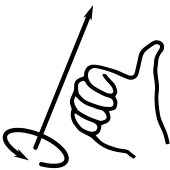
\includegraphics[scale=0.5]{curl_right_hand_rule}$$ If we curl our hands in the direction of rotation, we will know the direction in which the vector representing the rotation will point. This means that we can describe any give rotation in three-dimensional space with a vector.


This means that, when taking the curl of a three-dimensional vector field, our output will be a vector field describing the rotation of each vector. Computing three-dimensional curl is where the notation---del cross---comes in handy. 


Suppose 
$$
\mb{v}(x,\,y,\,z) =\left[\begin{array}{c}P(x,\, y,\, z)\\Q(x,\, y,\, z)\\ R(x,\,y,\,z)\end{array}\right].
$$
If we wanted to take the curl of $\mb{v}$, we would once again imagine crossing a vector of partial differential operators with $\mb{v}$. This is equivalent to imagining a determinant of a three-by-three matrix (which is only a notational trick, not mathematically proper):
\ba
\curl\mb{v}&=\det\left(\begin{array}{ccc}\hat{\imath}&\hat{\jmath}&\hat{k}\\\partial_x&\partial_y&\partial_z\\P&Q&R\end{array}\right)\\
&=\ihat\,(\partial_y R - \partial_z Q) - \jhat\,(\partial_x R - \partial_z P) + \khat \, (\partial_x Q- \partial_y P)
\end{align*}
This is the curl of a three dimensional vector fields with components $P$, $Q$,  and $R$. In column vector notation,
$$
\curl\mb{v} = \left[\begin{array}{c}\partial_y R - \partial_z Q\\-\partial_x R + \partial_z P\\ \partial_x Q- \partial_y P\end{array}\right]
$$
Since this concept of three-dimensional curl is a little more challenging than the concepts of divergence and two-dimensional curl, it is best to go through an example.

\begin{ex}Suppose we want to take the curl of 
$$
\mb{v}(x,\,y,\,z) =  \left[\begin{array}{c}  xy  \\  \cos z \\  z^2+y  \end{array}\right].
$$
We start by taking the following determinant
\ba
\curl \mb{v} &= \det\left(\begin{array}{ccc}\hat{\imath}&\hat{\jmath}&\hat{k}\\\partial_x&\partial_y&\partial_z\\xy&\cos z&z^2+y\end{array}\right)\\
&= \ihat\,(\partial_y (z^2+y) - \partial_z (\cos z)) - \jhat\,(\partial_x (z^2+y) - \partial_z (xy)) + \khat \, (\partial_x (\cos z)- \partial_y (xy)),
\end{align*}
and finish by computing partial derivatives:
\ba
\curl\mb{v}&= 
\boxed{ \ihat\,(1+\sin z) + \khat\,(-x)} \textrm{ or }\\
&= \boxed{ \left[\begin{array}{c}  1+\sin z  \\  0 \\  -x  \end{array}\right]}
\end{align*}\end{ex}




\subsection{The Laplacian}
 Suppose $f$ is a two dimensional function. The \textit{Laplacian} of $f$, denoted $\nabla^2 f$, outputs the divergence of the gradient of $f$.
$$
\nabla^2 f \equiv \divg \nabla f
$$
We know that the gradient operator returns a vector field of the vectors of steepest ascent. In this gradient field, vectors tend to diverge more when the point is a minimum, and less when it is a maximum. This fact only makes sense, since all vectors will be converging to a maximum and diverging from a minimum. Therefore, you can think of the Laplacian operator as measuring how much of a minimum a point is. We can also conclude that the Laplacian is equivalent to
$$
\nabla^2f\equiv\sum_i \partial_{x_ix_i}f.
$$


A function $f$ is a \textit{harmonic function} if and only if
$$
\nabla^2 f \equiv 0.
$$




\subsection{The Jacobian}
 For a transformation $L$, recall that the transformation is linear if and only if it satisfies the following two properties:
\begin{align*}
L(a\,\mb{v}) &= a\, L(\mb{v})\\
L(\mb{v} + \mb{w}) &= L(\mb{v}) + L(\mb{w})
\end{align*}
Also recall that we can represent a linear transformation by multiplying a matrix by a vector, where the $n$th column of the matrix corresponds to the new vector representation of the $n$th basis vector. Multivariable calculus moves beyond the scope of linear transformations, though. 


Suppose 
$$
\mb{r}\left(\vect{x}{y}\right) = \vect{x + \sin y}{y + \sin x}.
$$
This function is \textit{locally linear}, which roughly and graphically means that if you zoom in on a certain point, the transformation will seem linear near that point. So, if we call some point undergoing this transformation $\mb{x}$,
then there should be a two-by-two matrix by which you multiply $\mb{x}$ to represent the linear transformation that seemed to have taken place. Though we will not go through the details of deriving it, the matrix with this property is called the \textit{Jacobian matrix}. The Jacobian is also the matrix of $\mb{r}$'s first-order partial derivatives. Suppose we split $\mb{r}$ into two scalar-valued functions:
$$
\vect{r_1(x,\, y)}{r_2(x,\, y)} = \vect{x + \sin y}{y + \sin x}
$$
The Jacobian matrix of $\mb{r}$ is then
\ba
&=\left[\begin{array}{ccc}\partial_xr_1&\partial_yr_1\\\partial_xr_2&\partial_yr_2\end{array}\right]\\
&=\left[\begin{array}{ccc}1&\cos y\\\cos x&1\end{array}\right]
\end{align*}
If you wanted to find that matrix that is analogous to the transformation near $\mb{x}$, then you would simply evaluate the Jacobian at $\mb{x}$.


We know that taking the determinant of any two-by-two matrix is akin to answering the question, ``By what factor is a unit area changed after the transformation represented by that matrix?'' If we take the determinant of the Jacobian, we call it, rather unsurprisingly, the \textit{Jacobian determinant}. That tells us the factor by which a unit area changes in the neighbourhood of a certain point. So, if we wanted to determine (pun intended) the factor by which a unit area changes in the neighbourhood of $\mb{x}$, then we would take the determinant of $\mb{J}_{\mb{r}}$ evaluated at $\mb{x}$.





\section{Integrating multivariable functions}
\subsection{The line integral}
Suppose $\mb{r}$ parameterizes a curve $\gamma$ where $\mb{r}(a)$ and $\mb{r}(b)$ are the endpoints of $\gamma$. The \textit{line integral} of $\gamma$ is the area between $\gamma$ and a surface described by field $f$. The line integral of $\gamma$ along $f$ is defined as 
$$
\int_\gamma f(x,\, y)\diff{s} \equiv \int_a^b f(\mb{r}(t))\left|\frac{ d \mb{r}}{ d t}\right| \diff{t}.
$$


\begin{ex}Suppose 
$$
f(x,\, y) = xy
$$
and a curve $C$ is parameterized by $\mb{r}$, where
$$
\mb{r}(t) = \vect{\cos t}{\sin t}
$$
and
$$
0 \leqslant t \leqslant \frac{\pi}{2}.
$$
If we wanted to determine the line integral of $C$ along $f$, we simply use our definite integral definition and solve.
\ba
\int_C f(x,\, y)\diff{s} &= \int_{0}^{\pi/2} xy\, \left|\frac{ d \mb{r}}{ d t}\right|\diff{t}\\
&= \int_{0}^{\pi/2}xy \, \sqrt{\pars{ d x/ d t}^2 +\pars{ d y/ d t}^2 } \diff{t}\\
&=\int_{0}^{\pi/2} \cos(t)\sin(t) \sqrt{\pars{-\sin(t)}^2 + \pars{\cos(t)}^2} \diff{t}\\
&=\int_{0}^{\pi/2} \cos(t)\sin(t) \diff{t}
\end{align*}
If we let $u = \sin(t)$, then $ d u = \cos(t)\diff{t}$. Adjusting boundary conditions and evaluating,
\ba
\int_C f(\mb{r})\diff{s} &= \int_0^1 u \diff{u}\\
&= \frac{u^2}{2}\,\bigg|_0^1\\
&= \boxed{\frac{1}{2}}
\end{align*}
\end{ex}


% INCLUDE THIS EXAMPLE https://www.khanacademy.org/math/multivariable-calculus/integrating-multivariable-functions/line-integrals/v/line-integral-example-2-part-1?modal=1
\subsection{Line integrals and vector fields}
Recall that \textit{work} is defined as 
$$
W \equiv \mb{F} \cdot \mb{s}
$$
where $\mb{F} $ is force, $\mb{s}$ is displacement. This is, of course, equivalent to
$$
W \equiv F s\,\cos\theta
$$
where $F$ and $s$ are the magnitudes of the force and displacement, and $\theta$ is the angle between the direction of magnitude and force.


If $\mb{r}$ parameterizes some curve $\gamma$ that, for instance, represents the path of a particle in a vector field $\mb{v}$, then the work done on the particle by the field is
$$
W \equiv \int_\gamma \mb{v} \cdot  d \mb{r}.
$$

\begin{ex}
Suppose $\mb{v}$ is a vector field where 
$$
\mb{v}(x,\, y) = y\,\ihat - x\,\jhat
$$
and a curve $C$, representing a particle's path, is parametrized by 
\begin{align*}
x &= \cos t,\\
y&=\sin t
\end{align*}
where 
$$
0 \leqslant t \leqslant 2\pi.
$$
Let's say we want to determine the work done on the particle by the field. We start by determining $ d \mb{r}$.
\begin{align*}
\frac{d\mb{r}}{dt} &= -\sin(t)\, \ihat + \cos(t)\,\jhat\\
d\mb{r} &= -\sin(t)\diff{t}\, \ihat + \cos(t)\diff{t}\,\jhat
\end{align*}
We will then write $\mb{v}$ in terms of $t$.
\ba
\mb{v}(t) = \sin(t)\,\ihat - \cos(t) \,\jhat
\end{align*}
We now use our definite integral definition of the line integral.
\ba
\int_C \mb{v} \cdot d \mb{r}&= \int_0^{2\pi} -\sin^2(t)\diff{t} - \cos^2(t)\diff{t}\\
&= -\int _0^{2\pi} \pars{\sin^2(t) +\cos^2{t}}\diff{t}\\
&= -\int _0^{2\pi}\diff{t}\\
&= -t \,\bigg|_0^{2\pi}\\
&= \boxed{-2\pi\,\mathrm{J}}
\end{align*}
\end{ex}
% MAYBE ADD HOW REVERSE PARAMETERIZATION OF   C : x(t), y(t)   IS   -C : x(a+b-t), y(a+b-t)    AND HOW THEY ARE THE SAME FOR SCALAR FIELDS BUT - FOR VECTOR FIELDS


For a vector field $\mb{v}$ and two curves $\gamma_1$ and $\gamma_2$ on $\mb{v}$ with the same beginning and end points, the vector field is \textit{path independent} or \textit{conservative} if
$$
\int_{\gamma_1} \mb{v} \cdot d\mb{r} \equiv \int_{\gamma_2} \mb{v} \cdot d\mb{r}.
$$
Also, if $\mb{v}$ is the gradient of some scalar-valued function, then $\mb{v}$ is path independent.


A \textit{closed line integral}, denoted $\oint$, is a line integral that integrates a closed loop. As a corollary of the definition of path independence, if a vector field is path independent, then, for any closed curve on that field,
$$
\oint \mb{v} \cdot d\mb{r} \equiv 0.
$$
\begin{ex}
Evaluate
$$
I = \oint_C \pars{x^2 + y^2}\diff{x} + \pars{2xy}\diff{y}
$$
where $C$ is parameterized by
\ba
x &= \cos t,\\
y &=\sin t
\end{align*}
and 
$$
0 \leqslant t \leqslant 2\pi.
$$
Let us define a vector field
$$
\mb{v}(x,\, y) = \pars{x^2 + y^2}\, \ihat + \pars{2xy}\,\jhat.
$$
With that in mind,
$$
I = \oint_C \mb{v} \cdot d\mb{r}
$$
We can now determine whether or not $\mb{v}$ is conservative. If $F$ is the scalar-valued function whose gradient is $\mb{v}$, then we must take the partial antiderivatives with respect to $x$ and $y$.
\ba
\partial_x F &= x^2 + y^2\\
F &= \frac{x^3}{3} + xy^2 + f(y)
\end{align*}
Take the antiderivative with respect to $y$.
\ba
\partial_y F &=2xy\\
F &= xy^2 + g(x)
\end{align*}
Align both results.
\ba
F(x,\, y) =  \frac{x^3}{3} + xy^2
\end{align*}
Since $\mb{v}$ is the gradient of some scalar-valued function, it is conservative, and therefore,
$$
I = \boxed{0}
$$
\end{ex}




\subsection{The double integral}
The \textit{double integral} is used to determine the area under a surface. 
\begin{ex}
Suppose 
$$
f(x,\, y) = xy^2
$$
and we want to find the area under $f$ for
$$
0 \leqslant x \leqslant 2\  \mathrm{ and }\  0 \leqslant y \leqslant 1.
$$ We would use a double integral, like so,
$$
\int_0^1\int_0^2 xy^2\diff{x}\diff{y},
$$
evaluating the inner integral first.
\ba
\ &\int _0^1 {\frac{x^2}{2}y^2\,\bigg|_0^2}\diff{y}\\
= \ &\int _0^1 2y^2 \diff{y}\\
=\ & \frac{2y^3}{3} \,\bigg|_0^1\\
=\ &\boxed{\frac{2}{3}}
\end{align*}
\end{ex}
It does not matter whether we integrate with respect to $x$ or $y$ first.
\begin{ex}
Let 
$$
f(x,\, y) = xy^2.
$$
Let's say we want to find the area under $f$ for
$$
0 \leqslant x \leqslant 1 \textrm{ and } y = x^2.
$$
This would form some parabolic arc underneath the surface. To evaluate, we would set up our integral like so
$$
\int_0^1 \int_0^{x^2} xy^2 \diff{y}\diff{x},
$$
then evaluate.
\ba
\ &\int_0^1 {\frac{xy^3}{3}\,\bigg|_0^{x^2}} \diff{x}\\
= \ &\int_0^1 \frac{x^7}{3} \diff{x}\\ 
=\ &\frac{x^8}{24}\,\bigg|_0^1\\
= \ &\boxed{\frac{1}{24}}
\end{align*}
\end{ex}
Always make sure your inner integral is the one with the variable boundary.


There is a more compact way to write a double integral. If the domain of the area you want to integrate is $D$ and the area itself is $A$, then the double integral can be written as
$$
\iint_D f(x,\,y)\diff{A}.
$$\\


We can use polar coordinates to make integrations with rotational symmetry, like a disc or functions containing $x^2 + y^2$, a lot easier. A few conversions are necessary to utilize it:
\ba
x^2 + y^2 &= r^2\\
dA &= r\diff{\theta}\diff{r}
\end{align*}
\begin{ex}
Evaluate 
$$
I = \iint_{\bb{R}^2} e^{-\pars{x^2+y^2}}\diff{A}.
$$
We know that
$$
I = \int_{-\infty}^\infty \int_{-\infty}^{\infty} e^{-\pars{x^2+y^2}}\diff{x}\diff{y}.
$$
Convert to polar coordinates, then evaluate the integrals.
\ba
I &= \int_0^\infty \int_0^{2\pi} e^{-r^2} r\diff{\theta}{\diff{r}}\\
&= \int_0^\infty e^{-r^2}r\,\theta\,\bigg|_0^{2\pi}\diff{r}\\
&= 2\pi\int_0^\infty e^{-r^2}r\diff{r}
\end{align*}
If we let $u = -r^2$, then $-\frac{1}{2}\diff{u}=r\diff{r}$. 
\ba
I &= -\frac{1}{2}\,2\pi\int_0^\infty e^{u}\diff{u}\\
&= -\pi \, e^u\,\bigg|_0^\infty\\
&=\boxed{\pi}
\end{align*}
\end{ex}


\subsection{The triple integral}

%MAKE THIS LESS VERBOSE AND MORE READABLE

The \textit{triple integral} is the three-dimensional analogue of the double integral. It is worth asking what use the triple integral serves, since we can figure out three-dimensional areas using the double integral. The triple integral, however, can help us determine the mass of a certain three-dimensional figure if its density varies. 
\begin{ex}
Suppose we want to find the mass of the area bounded in the positive octant between a plane described by
$$
2x + y + 3z = 6
$$
and another plane described by 
$$
z = 2
$$
that has a density function
$$
\rho(x,\,y,\,z) = x^2yz
$$
in terms of $\mathrm{kg}/\mathrm{m}^3$. 
We need to determine boundaries for our integrals. We solve for $dz$'s boundaries first. The bottom boundary is 
\ba
3z &= 6 - 2x - y\\
z&=2 - \frac{2x}{3} - \frac{y}{3}.
\end{align*}
We also know the top boundary is $z = 2$, since that's where the second plane is. For $dx$'s boundaries, we will need to see a projection of the volume in two dimensions. The lower boundary is 0 since we are bounded by the axis. The upper boundary must be in terms of $y$. We set $z=0$ since $dz$'s boundaries are the innermost, and determine the equation of the upper boundary.
\ba
2x + y &= 6\\
x &= 3 - \frac{y}{2}
\end{align*}
$dy$'s boundaries can only be numerical. Therefore, from the projection, its lower boundary is 0 and its upper boundary is 6. We can now set up the triple integral to determine the mass.
\ba
m &= \int_0^6\int_0^{3 - y/2}\int_{2 - {2x}/{3} - {y}/{3}}^{2} \rho(x,\,y,\,z) \diff{z}\diff{x}\diff{y}\\
&= \int_0^6\int_0^{3 - y/2}\int_{2 - {2x}/{3} - {y}/{3}}^{2} x^2yz \diff{z}\diff{x}\diff{y}\\
&= \boxed{30.8571 \textrm{ kg}}
\end{align*}
\end{ex}



\subsection{The surface integral}
The \textit{surface integral} allows us to find the area of a surface; it is the double integral analogue of the line integral. To calculate a surface's surface integral, we must parameterize the surface.
\begin{ex}
The parameterization of a torus is
$$
\mb{r}(s,\,t) = \pars{\pars{b +a\,\cos(s)}\,\sin(t)}\ihat + \pars{\pars{b+a\,\cos(s)}\,\cos(t)}\jhat + \pars{a\,\sin(s)}\khat
$$
where $a$ is the radius of the torus' cross-sectional circles, where $b$ is the distance from the torus' centre to the centre of the cross sections, and where
$$
0\leqslant s \leqslant 2 \pi, \  0 \leqslant t\leqslant 2\pi.
$$
Determine the surface area of a torus $\Sigma$. 


We will set up the surface integral as a double integral, like so
$$
\iint_\Sigma d\Sigma.
$$
Think of $d\Sigma$ as a patch of area on the surface. It has to move in two directions to capture all of the surface area (up/down and left/right in the case of the torus), hence the double integral. We will not derive another expression for $d\Sigma$ from the bottom up, but recall that the magnitude of the cross product of two vectors is the area of the parallelogram formed by the two vectors. We can think of $d\Sigma$ as the cross product of two vectors, specifically, the cross product of the partial derivatives of $\mb{r}$. We can then represent the surface integral above as 
$$
\iint_R |\partial_s\mb{r} \times \partial_t\mb{r}|\diff{s}\diff{t}
$$
where $R$ is the domain of $\mb{r}$. Let's begin with the partial derivative with respect to $s$.
$$
\partial_s\mb{r}  = -\pars{a\,\sin(t)\sin(s)}\ihat - \pars{a\,\cos(t)\sin(s)}\jhat + \pars{a\,\cos(s)}\khat
$$
Then with respect to $t$.
$$
\partial_t\mb{r} \pars{\pars{b + a\,\cos(s)}\,\cos(t)}\ihat - \pars{\pars{b+a\,\cos(t)}\,\sin(t)}\jhat +0\,\khat
$$
We will now determine the cross product of these two partial derivatives.
\ba
\partial_s\mb{r} \times \partial_t\mb{r} = &\cdets{-a\sin(t)\sin(s)}{-a\cos(t)\sin(s)}{a\cos(s)}{\pars{b + a\cos(s)}\cos(t)}{-\pars{b+a\cos(s)}\sin(t)}{0}\\
= &\pars{{a\cos(s) \cdot \pars{b+a\cos(s)}\sin(t) }} \ihat + \pars{ a\cos(s)\cdot\pars{b + a\cos(s)}\cos(t) } \jhat \\ &+ \pars{a\sin(t)\sin(s)\cdot\pars{b+a\cos(s)}\sin(t)   +    {a\cos(t)\sin(s)}\cdot\pars{b + a\cos(s)}\cos(t) }\khat\\
= &(b + a\cos(s))\pars{\pars{a\cos(s)\sin(t)}\ihat + \pars{a\cos(s)\cos(t)}\jhat + \pars{a\sin(s)\pars{\sin^2(t) + \cos^2(t)}}\khat}\\
= &(b + a\cos(s))\pars{\pars{a\cos(s)\sin(t)}\ihat + \pars{a\cos(s)\cos(t)}\jhat + \pars{a\sin(s)}\khat}
\end{align*}
We will now determine the magnitude of the above expression.
\ba
|\partial_s\mb{r} \times \partial_t\mb{r}| &= (b + a\cos(s))\sqrt{a^2\cos^2(s)\sin^2(t) + a^2\cos^2(s)\cos^2(t) + a^2\sin^2(s)}\\
&=  (b + a\cos(s))\sqrt{\pars{a^2\cos^2(s)}\pars{\sin^2(t) +\cos^2(t)} + a^2\sin^2(s)}\\
&= (b + a\cos(s))\sqrt{a^2\pars{\cos^2(s) +\sin^2(s)}} \\
&= (b+a\cos(s))\,a\\
&= ab + a^2\cos(s)
\end{align*}
We can now put this into the double integral.
\ba
\iint_\Sigma d\Sigma &= \int_0^{2\pi}\int_0^{2\pi} |\partial_s\mb{r} \times \partial_t\mb{r}|\diff{s}\diff{t}\\
&= \int_0^{2\pi}\int_0^{2\pi} ab + a^2\cos(s) \diff{s}\diff{t}\\
&= \int_0^{ 2\pi}  abs + a^2\sin(s)\,\bigg|_0^{2\pi}\diff{t}\\
&= 2\pi\int_0^{2\pi} ab \diff{t}\\
&= 2\pi \, abt\,\bigg|_0^{2\pi}\\
&= \boxed{4\pi^2 ab}
% I've never smiled so much
\end{align*}
\end{ex}


\begin{ex}
Determine
$$
I = \iint_\Sigma x^2 \diff{\Sigma}
$$
where $\Sigma$ is the unit sphere. 


The unit sphere is parameterized by 
$$
\mb{r}(s,\,t) = \pars{\cos(t)\cos(s)}\ihat + \pars{\cos(t)\sin(s)}\jhat + \pars{\sin(t)}\khat
$$
where 
$$
0\leqslant s \leqslant 2\pi, \  -\frac{\pi}{2} \leqslant t \leqslant \frac{\pi}{2}.
$$
Take the partial derivative with respect to $s$.
$$
\partial_s\mb{r} = -\pars{\cos(t)\sin(s)}\ihat + \pars{\cos(t)\cos(s)}\jhat + {0}\khat
$$
Then with respect to $t$.
$$
\partial_t\mb{r} = -\pars{\sin(t)\cos(s)}\ihat -\pars{\sin(t)\sin(s)}\jhat + \pars{\cos(t)}\khat
$$
To save space, the steps in taking the cross product will not be shown. This is left as an exercise.
$$
\partial_s\mb{r} \times \partial_t\mb{r} = \pars{\cos^2(t)\cos(s)}\ihat + \pars{\cos^2(t)\sin(s)}\jhat + \pars{\cos(t)\sin(t)}\khat
$$
Now, we take the magnitude of that result.
$$
|\partial_s\mb{r} \times \partial_t\mb{r}| = \cos(t)
$$
We now know that $d\Sigma = \cos(t)\diff{s}\diff{t}$. We must also express $x^2$ in terms of our parameters. Simple calculation shows that $x^2 = \cos^2(t)\cos^2(s)$. Let us wrap this up.
\ba
I &= \int_{-\pi/2}^{\pi/2} \int_0^{2\pi} \cos^2(t)\cos^2(s)\cos(t)\diff{s}\diff{t}\\
&=  \int_{-\pi/2}^{\pi/2}\cos^3(t)\diff{t} \int_0^{2\pi} \cos^2(s)\diff{s}\\
&= \int_{-\pi/2}^{\pi/2}\cos(t) - \cos(t)\sin^2(t) \diff{t} \int_0^{2\pi} \frac{1}{2} + \frac{1}{2}\cos(2s)\diff{s}\\
&= \pars{\sin(t) - \frac{\sin^3(t)}{3}}\,\bigg|_{-\pi/2}^{\pi/2}   \pars{\frac{t}{2} + \frac{\sin(2s)}{4}}\,\bigg|_0^{2\pi}\\
&= \boxed{\frac{4\pi}{3}}
\end{align*}
\end{ex}




\subsection{Flux}
Suppose $\rho$ is a three-dimensional function of mass density and $\mb{v}$ is a function of velocity. Let 
$$
\mb{F} = \rho\mb{v}
$$
and suppose we have the surface integral over some surface $\Sigma$
$$
\iint_\Sigma \mb{F} \cdot \mb{n}\diff{\Sigma}.
$$
where $\mb{n}$ is the unit normal vector at each point. $\mb{F}$ is in terms of $\mathrm{kg}/\mathrm{m}^2\mathrm{s}$ and $d\Sigma$ is in terms of $\mathrm{m}^2$, so the surface integral is in terms of $\mathrm{kg}/\mathrm{s}$; it answers the question ``how much mass is travelling through $\Sigma$ at a moment in time?'' This is, essentially, \textit{flux} through a two-dimensional surface.


We need to know how to construct a unit normal vector at any point on the surface. We assume that $\Sigma$ can be parameterized by $\mb{r}(u,\, v)$. It is, quite simply,
$$
\mb{n}(u,\,v) = \frac{\partial_u\mb{r}\times\partial_v\mb{r}}{|\partial_u\mb{r}\times\partial_v\mb{r}|}.
$$
This makes sense; $\partial_u\mb{r}$ and $\partial_v\mb{r}$ are tangent to $\Sigma$, and the cross product will output a vector perpendicular to both---normal to $\Sigma$.


If we refer back to the surface integral at the beginning of this subsection, we can now determine that it is equivalent to the double integral
$$
\iint_R \mb{F} \cdot \pars{\partial_u\mb{r}\times\partial_v\mb{r}} \diff{u}\diff{v}
$$
where $R$ is the domain of $\mb{r}$.


Though we have been uniform in our notation heretofore, another way to write the first surface integral is
$$
\iint_\Sigma \mb{F} \cdot \diff{\mb{\Sigma}}.
$$ 



\section{Green's, Stokes', and divergence theorems}

\subsection{Types of regions in $\bb{R}^3$}
A \textit{type I region} $R$ is defined as
$$
 \{ (x,\,y,\,z) \, |\, (x,\,y) \in D,\, f_1(x,\, y) \leqslant z \leqslant f_2(x,\,y)\}
$$
where $D$ is the domain defined by $R$. This, essentially, means that if we take the cross section of $R$ on the $yz$ plane, each $y$ would have at most two corresponding $z$s. 


A \textit{type II region} $R$ is defined as 
$$
 \{ (x,\,y,\,z) \, |\, (y,\,z) \in D,\, f_1(y,\, z) \leqslant x \leqslant f_2(y,\, z)\}
$$
where $D$ is the domain defined by $R$. This means that if we take the cross section of $R$ on the $zx$ plane, each $z$ would have at most two corresponding $x$s.


A \textit{type III region} $R$ is defined as 
$$
 \{ (x,\,y,\,z) \, |\, (x,\,z) \in D,\, f_1(x,\, z) \leqslant y \leqslant f_2(x,\, z)\}
$$
where $D$ is the domain defined by $R$. This means that if we take the cross section of $R$ on the $xy$ plane, each $x$ would have at most two corresponding $y$s.





\subsection{Green's theorem}
Let $C$ be a closed path and let $\mb{p}$ be a vector field such that
$$
\mb{p}(x,\,y) = P(x,\,y)\ihat.
$$
Suppose we want to determine
$$
I_1 = \oint_C \mb{p}\cdot d\mb{r}.
$$
We know that
$$
I_1 = \oint_C P(x,\,y)\diff{x}
$$
since there is no $y$ component. Let $a$ and $b$ be the minimum and maximum $x$ components of $C$ respectively, and let $y_1$ and $y_2$ be functions of $x$, one of which describing the curve from $a$ to $b$, and the other describing the curve from $b$ to $a$. Therefore,
\ba
I_1 &= \int_a^bP(x, \,y_1(x))\diff{x} + \int_b^a P(x, \,y_2(x))\diff{x}\\
&= \int_a^b P(x, \,y_1(x)) - P(x, \,y_2(x))\diff{x}\\
&= -\int _a^b P(x, \,y_2(x)) - P(x, \,y_1(x))\diff{x}\\
&= - \int_a^b P(x,\,y) \,\bigg|_{\,y\,=\,y_1(x)}^{\,y\,=\,y_2(x)}\diff{x}
\end{align*}
Assuming that $P$ has a partial derivative,
\ba
I_1 &= -\int_a^b\int_{y_1(x)}^{y_2(x)}\partial_yP\diff{y}\diff{x}.
\end{align*}
We have, so far, concluded that
$$
\oint_C P(x,\,y)\diff{x} \equiv -\iint_R \partial_y P\diff{y}\diff{x},
$$
where $R$ is the region enclosed by $C$.


Let $\mb{q}$ be a vector field such that
$$
\mb{q}(x,\, y) = Q(x,\,y)\jhat.
$$
Suppose we want to determine
$$
I_2 = \oint_C \mb{q}\cdot d\mb{r}.
$$
If we follow the same logic as we did originally, we will find that 
$$
I_2 = \oint_C Q(x,\,y)\diff{y},
$$
and eventually,
$$
\oint_C Q(x,\,y)\diff{y} = \iint_{R} \partial_x Q \diff{x}\diff{y}.
$$


Let
$$
\mb{F}(x,\,y) = P(x,\,y)\ihat + Q(x,\,y)\jhat
$$
and let $\Omega$ be some closed path on $\mb{F}$. As a result of what we found previously,
$$
\oint_\Omega \mb{F}\cdot d\mb{r} \equiv \iint_R \partial_x Q - \partial_y P \diff{A}
$$
where $dA = dx\,dy$, where $R$ is the region enclosed by $\Omega$, and where the path of integration along $\Omega $ is counterclockwise. This is \textit{Green's theorem}. As a corollary, if $\mb{F}$ is conservative, then
$$
\partial_x Q - \partial_y P \equiv 0.
$$
\begin{ex} Determine
$$
I = \oint_C \pars{x^2-y^2}\diff{x} + 2xy\diff{y}
$$
where $C$ bounds a region $R$ such that 
$$
0\leqslant x\leqslant 1,\ 2x^2\leqslant y \leqslant 2x.
$$
By Green's theorem, 
\ba
I &=  \iint_R \partial_y\pars{x^2-y^2} - \partial_x\pars{2xy}\diff{A}\\
&= \int_0^1 \int_{2x^2}^{2x} 4y \diff{y}\diff{x}\\
&= \int_0^1 2y^2\,\bigg|_{2x^2}^{2x} \diff{x}\\
&= \int_0^18x^2-8x^4\diff{x}\\
&= \frac{8x^3}{3} - \frac{8x^5}{5}\,\bigg|_{0}^1\\
&= \boxed{\frac{16}{15}}
\end{align*}
\end{ex}






\subsection{Stokes' theorem}
Let $\Sigma$ be a surface bounded by $C$ and let $\mb{F}$ be a vector field in $\Sigma$'s neighbourhood. \textit{Stokes' theorem} says that 
$$
\oint_C\mb{F}\cdot d\mb{r} \equiv \iint_\Sigma \pars{\curl{\mb{F}}}\cdot d\mb{\Sigma}.
$$
We can rewrite the right side of the equality to be 
$$
\iint_\Sigma \pars{\curl{\mb{F}}} \cdot \mb{n}\diff{\Sigma}.
$$\\


Suppose that 
$$
\mb{F} = P(x,\,y)\ihat+ Q(x,\,y)\jhat.
$$
If we take the rewritten double integral before of $\mb{F}$, we find something interesting. Let $C$ enclose a two-dimensional region $R$ in three dimensions. Start with computing the curl (the steps of which are presented as an exercise).
$$
\curl{\mb{F}} = \pars{\partial_xQ -\partial_yP}\khat
$$
Since $\khat$ is the same as $\mb{n}$, we can say that
$$
\oint_C\mb{F}\cdot d\mb{r} \equiv \iint_R \partial_x Q - \partial_y P \diff{A}.
$$
This equality shows how, fundamentally, Green's theorem and Stokes' theorem are related.


The normal vector of a surface can point in two directions; ``inwards'' or ``outwards'' relative to the surface. Similarly, the boundary of a surface can be made clockwise or counterclockwise. For Stokes' theorem to hold, these orientations have to be consistent. If you are familiar with the right hand rule described in the subsection on curl, that right hand rule describes the direction of the normal vector depending on the direction of integration and vice versa.


There are some conditions for Stokes' theorem. Let $\Sigma$ be the surface over which we are integrating. Firstly, $\Sigma$ must be \textit{piecewise smooth}, which means that, if $\Sigma$ is not continuous and differentiable everywhere, we can break $\Sigma$ up into pieces that are continuous and differentiable everywhere. Let $C$ be the boundary of $\Sigma$. $C$ must be \textit{simple}, meaning $C$ does not intersect itself, closed, and piecewise smooth.

\begin{ex}
Let $C$ be the boundary formed by the intersection of the plane $y+z=2$ and $x^2+y^2=1$. Let 
$$
\mb{F} = -y^2\,\ihat +x\,\jhat +z^2\,\khat.
$$
Determine 
$$
I = \oint_C \mb{F} \cdot d\mb{r}
$$
using Stokes' theorem if $C$ is integrated in a counterclockwise direction. 



Let $\Sigma$ be the region bounded by $C$. We know that
$$
I = \iint_\Sigma \pars{\curl{\mb{F}}} \cdot \mb{n}\diff\Sigma.
$$
The steps of parameterizing $C$ are an exercise. $C$ can be parameterized by 
$$
\mb{s} (r,\,\theta) = r\cos\theta\,\ihat + r\sin\theta\,\jhat +\pars{2-r\sin\theta}\khat
$$
where 
$$
0 \leqslant \theta \leqslant 2\pi,\ 0\leqslant r\leqslant 1.
$$
We can rewrite $\mb{n}\diff{\Sigma}$ as $\pars{\partial_r\mb{s} \times \partial_\theta\mb{s}}\diff\theta\diff r$. We can confirm that this cross product will point in the direction we need by the right hand rule for the cross product and the counterclockwise nature of $C$. Take the cross product.
\ba
\partial_r\mb{s} \times \partial_\theta\mb{s} &= \cdets{\cos\theta}{\sin\theta}{-\sin\theta}{-r\sin\theta}{r\cos\theta}{-r\cos\theta}\\
&= r\,\jhat + r\,\khat
\end{align*}
We now have to evaluate the curl of $\mb{F}$.
\ba
\curl{\mb{F}} &= \cdet{-y^2}{x}{z^2}\\
&= \pars{1+2y}\khat\\
&= \pars{1+2r\sin\theta}\khat
\end{align*}
We can now evaluate $I$.
\ba
I &= \int_0^1\int_0^{2\pi}\pars{\pars{1+2r\sin\theta}\khat} \cdot \pars{r\,\jhat + r\,\khat} \diff\theta\diff r\\
&=\int_0^1\int_0^{2\pi} r+2r^2\sin\theta \diff\theta\diff r\\
&= \int_0^1 r\theta - 2r^2\cos\theta\,\bigg|_0^{2\pi}\diff r\\
&= \int_0^1 2\pi r \diff{r}\\
&= \pi r^2\,\bigg|_0^1\\
&= \boxed{\pi}\\
\end{align*}
\end{ex}

\subsection{Divergence theorem}
Let $R$ be a simple three-dimensional region. Let $\Sigma$ be the boundary of $R$. If $\mb{F}$ is a vector field in the neighbourhood of $R$, the flux through $\Sigma$ is 
$$
\oiint_\Sigma\pars{ \mb{F}\cdot\mb{n}}\diff\Sigma.
$$
We can think of this flux as a sum of divergences in $R$. By this statement, \textit{divergence theorem} states that 
$$
\oiint_\Sigma\pars{ \mb{F}\cdot\mb{n}}\diff\Sigma \equiv \iiint _R \pars{\divg{\mb{F}}} \diff V.
$$
\begin{ex}
Suppose $R$ is a simple three-dimensional region such that $-1\leqslant x\leqslant 1$, $z = 1-x^2$, and $y=2-z$. If $$
\mb{F} = \pars{\frac{1}{2}x^2+ e^{\cos zy}}\ihat + \pars{yx + \ln |z|}\jhat + \tan(xy)\,\khat,
$$
what is the flux of $\mb{F}$ through $R$?


We know from divergence theorem that the flux is nothing but 
$$
I = \iiint_R \pars{\divg{\mb{F}}} dV.
$$
Calculate the divergence.
\ba
\divg{\mb{F}} = 2x
\end{align*}
We can now evaluate the triple integral.
\ba
I &= \int_{-1}^1 \int_0^{1-x^2} \int_0^{2-z} 2x\diff{y}\diff{z}\diff{x}\\
&= \int_{-1}^1 \int_0^{1-x^2} 2xy \,\bigg|_0^{2-z}\diff{z}\diff{x}\\
&=  \int_{-1}^1 \int_0^{1-x^2} 2x(2-z) \diff{z}\diff{x}\\
&= \int_{-1}^1 2x\pars{2z - \frac{z^2}{2}}\,\bigg | _0^{1-x^2} \diff{x}\\
&= \int_{-1}^1 3x - 2x^3 - x^5\diff{x}\\
&= \frac{3x^2}{2} - \frac{x^4}{2} -\frac{x^6}{6}\,\bigg|_{-1}^1\\
&= \boxed{0}
\end{align*}
\end{ex}

% PROOF TOO HAND-WAVY
\iffalse
\bp
Let $\varpi$ be a simple, solid region enclosed by a surface $\Sigma$. Let $\mb{F}= P\,\ihat + Q\,\jhat + R\,\khat$ be a vector field in the neighbourhood of $\varpi$. We know that
$$
\oiint_\Sigma (\mb{F}\cdot\mb{n}) \diff\Sigma = \oiint_\Sigma P(\ihat\cdot\mb{n}) \diff\Sigma + \oiint_\Sigma Q(\jhat\cdot\mb{n}) \diff\Sigma + \oiint_\Sigma R({\khat\cdot\mb{n}}) \diff\Sigma.
$$
Also,
$$
\iiint_\varpi (\divg{\mb{F}}) \diff{V} =  \iiint_\varpi  \partial_xP   \diff{V} + \iiint_\varpi  \partial_yQ   \diff{V}+ \iiint_\varpi  \partial_zR   \diff{V}.
$$
Since $\varpi$ is simple, it is also a type I, a type II, and a type III region. If $\Sigma$ can be separated into three (for instance) smooth regions, $\Sigma_1$, $\Sigma_2$, and $\Sigma_3$, then 
$$
\oiint_{\Sigma} R({\khat\cdot\mb{n}}) \diff\Sigma = \oiint_{\Sigma_1} R({\khat\cdot\mb{n}}) \diff\Sigma + \oiint_{\Sigma_2} R({\khat\cdot\mb{n}}) \diff\Sigma + \oiint_{\Sigma_3} R({\khat\cdot\mb{n}}) \diff\Sigma
$$
\ep
\fi
 
\end{document}

%RELATE EVERYTHING TO FLUX WHEN TIME ALLOWS
hello \darkness my \old{friend}!^{\frac{1}{2}}